\section{Кравчук Никита - Вклады в иностранные банки}
Бюджет: 100.000 евро \\

\subsection{Мотивация}
Одна из проблем, с которой столкнутся мои коллеги - конвертация денег из одной валюты в другую. В связи с этим возникла идея избежать этих расходов
и, оставив деньги в 

\subsection{Покупка квартиры}
В этом пункте содержится много подводных камней. Какую сумму стоит отложит на ремонт/отделку квартиры/непредвиденные расходы? Какую квартиру лучше покупать 1 или 2-х комнатную? Каким образом должна быть расположена квартира? \\

Чтобы как-то определиться с этими вопросами, нужно понять, кто является "целевой аудиторией", т.е. будет снимать квартиру. Так как Москва - столица, потребность в аренде возникает у людей, которые приехали сюда работать. Поэтому, наиболее подходящей будет квартира, которая находится в пределах МКАД, в шаговой доступности от метро. Наличие поблизости дополнительной инфраструктуры, типа парковок, школ, поликлиник будет плюсом. \\

Основные потери видятся только в результате инфляции, поэтому подберем стоимость квартиры таким образом, чтобы ее компенсировать. Так же возможны потери из-за налогов, "простоя" квартиры (когда нет арендаторов), из-за продажи. Для простоты, что-то из этого вынесем в "необходимые расходы".\\

Если обозначить среднюю инфляцию как $I$, то за $n$ лет убыток от нее будет составлять $(1-(1-I)^{n})$ от общей суммы. Рассчитаем общий убыток: если за $P$ обозначить стоимость покупки квартиры, за $V$ обозначить некоторые "необходимые расходы", то в результате инфляции останется только сумма равная $P*(1-(1-I)^{n}) + V$ \\
Если считать, что квартиру можно сдать по цене средней цене $P_{avg}$ за месяц, то доход, полученный от сдачи квартиру в аренду будет составлять $12*n*K*p_{avg}$, где $K$ - коэффициэнт, зависящий от налогов .\\ Для того, чтобы не уйти в минус, нужно приравнять эти два выражения, получаем:
\begin{equation}
P*(1-(1-I)^{n}) + V = 12*n*K*p_{avg}
\end{equation}

\begin{equation}
P = \frac{12*n*K*p_{avg} - V}{1-(1-I)^{n}}
\end{equation}

Будем выбирать из четырех типов квартир:
\begin{enumerate}
	\item Однокомнатная новостройка
	\item Однакомнатная вторичная
	\item Двухкомнатная новостройка
	\item Двухкомнатная вторичная
	
\end{enumerate}

\begin{center}
	\begin{tabular}{ | l | l | l | l|}
	\hline
    \textbf{№} & \textbf{V} & \textbf{$p_{avg}$} & \textbf{P}\\ \hline
    1 & 600k & 32000 & 5835052 \\ \hline
    2 & 400k & 32000 & 6719150 \\ \hline
    3 & 800k & 45000 & 8398938 \\ \hline
    4 & 600k & 45000 & 9283037 \\ \hline
	\end{tabular}
\end{center}

Ближе всего к нужно сумме находится 4-ый вариант - двухкомнатная вторичная (не новостройка) квартира, её выберем в качестве окончательного варианта.
На сайте https://cian.ru можно найти довольно много квартир, удовлетворяющих критериям

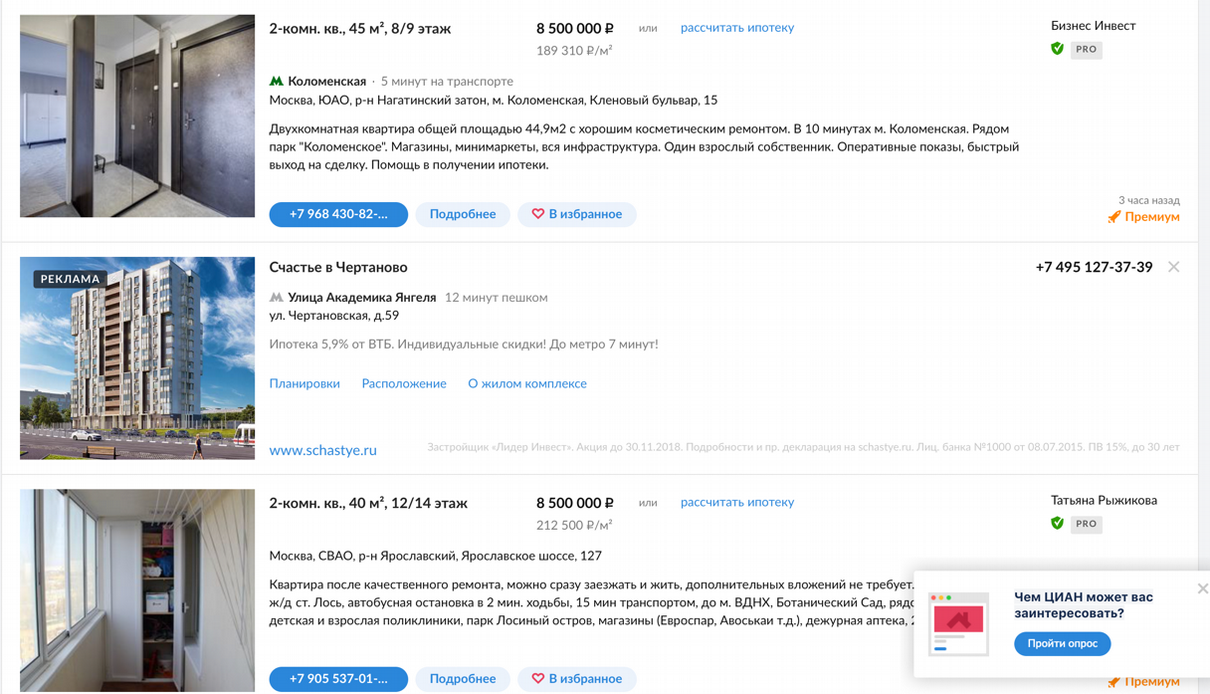
\includegraphics[width=16cm]{pics/ruslan/1.png}
На сколько сейчас выгодно покупать жилье. Если рассмотреть граффик за последние несколько лет, видно, что с 2015г. цена жилья идет вниз.
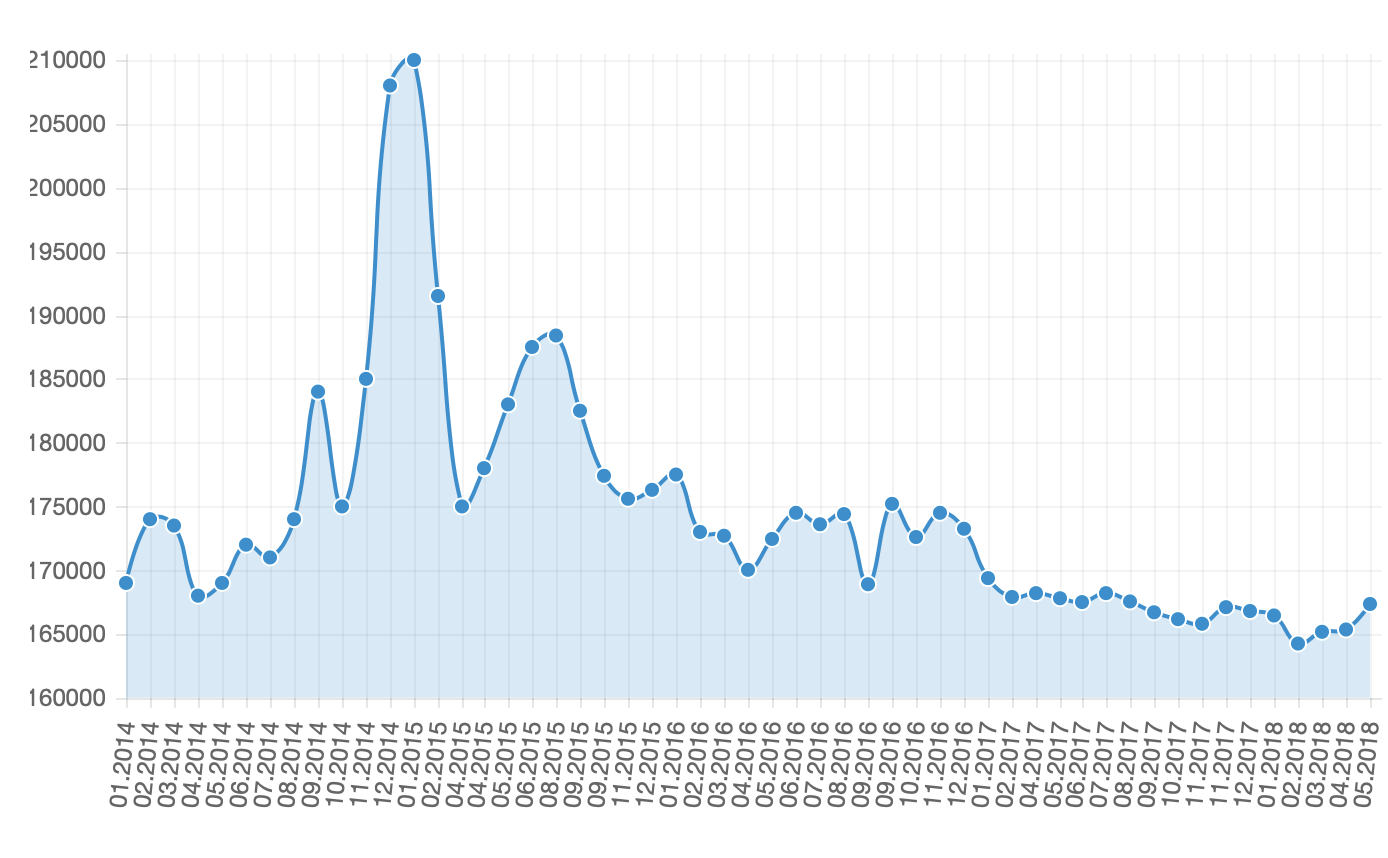
\includegraphics[width=14.5cm]{pics/ruslan/2.png}
Снижение цен на недвижимость случалось и ранее, - особенно после кризисов 1998 и 2008 гг. Цена падала, но через некоторое, довольно небольшое время, возвращалась к прежнему уровню. Сейчас же идет затяжное снижение. По прогнозам некоторых экспертов, цена на недвижимость продолжит снижаться, и к 2024 г. упадет еще ~ 10\% от текущего уровня. Будем опираться на эту цифру, при рассчете убытков в худшем случае.

\subsection{Сдача жилья в аренду}
Здесь так же много различных нюансов. Например, может случится так, что сдавать квартиру на длительный срок не получится. Смена и поиск арендаторов займут некоторое время. К тому же в каждый месяц, спрос на жилье не одинаков (как правило выше осенью, и ниже летом). Может случиться так, что сдать в аренду по средней цене не получится, тогда надо либо ждать, либо дополнительно сбрасывать цену. Это тоже доставляет убытки. \\
На графике приведен средний спрос на аренду двухкомнатной квартиры в Москве, по месяцам.

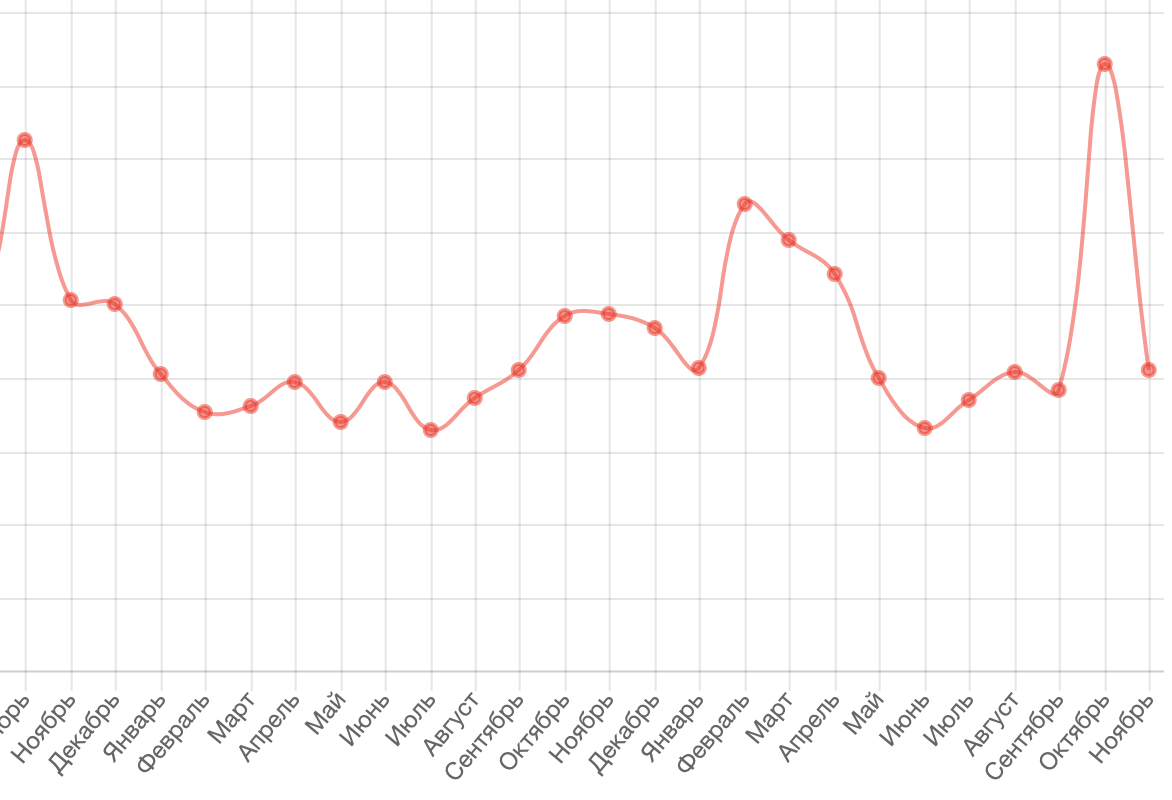
\includegraphics[width=14.5cm]{pics/ruslan/3.png}

\subsection{Продажа квартиры}
Тут стоит учитывать, что практически никогда нельзя сразу продать квартиру за ее рыночную стоимость.Для поиска покупателя, оформления соответствующих бумаг нужно время - обычно это занимает 4-6 месяцев. Можно срочно продать квартиру риелторам, но при этом теряется около 10\% ее цены, что менее выгодно по сравнению с обычным вариантом. Если начать поиск покупателя за 6 месяцев до окончания срока, то максимальные убытки будут в том случае, если он сразу найдется. Т.е. теряются 6 месяцев оплаты, но по сравнению с 10\% эта довольно незначительная сумма.

\subsection{Оценка убытков}
На каждом из следующих этапов возможны убытки:
\begin{itemize}
	\item На обмене валют. 3\% - в обе стороны
	\item Не будет арендаторов. Убыток ~ 5\%
	\item Потеря при продаже квартиры (из-за снижения цен на жилье) ~ 10\%, 3\% из-за сроков продажи
\end{itemize}
Потери в худшем случае составят: 3\% + 5\% + 10\% + 3\% = 21\%
На самом деле это не так плохо: потери от инфляции (5\% в год) за пять лет составят 22.6\%. Если ничего не делать, эти потери будут неизбежны, а приведенная оценка в 21\% - это оценка в худшем случае, вероятный исход скорее всего будет лучше.
Итого: получится сохранить как минимум 140*0.79 = 110.6 тысяч евро из 140